\section{Optimizations}

Modern SAT solvers use many advanced optimizations and heuristics to improve the solving time.
However these are usually designed for general problem instances.
With additional knowledge about a specific problem we can try to come up with better rules which lead to decrease of solving time.

In this chapter we will describe several optimizations that we implemented and evaluated.
Some of these involve a simple change in output instance generation, others involve changes to the SAT solvers themselves.

%TODO vsetko poriadne odmerat, otestovat a spisat
%TODO sem dat: xor klauzule, xor arita
%TODO spravit este: espresso minimizer
%TODO nech je toho dost, povymyslat dalsie?

\subsection{XOR clauses}
TODO ~1pgs

\subsection{Merging operators}
TODO ~0.5pgs

\subsection{Truth table minimization}
TODO ~1pgs + nejake porovnania velkosti a rychlosti

\subsection{Branching order}
\label{sec:branching-order}
%TODO nossum/soos mailing list cite; is it in text?; more references to literature

The most important heuristic in a SAT solver is the decision which unassigned variable to pick next.
A bad order might assign randomly picked values to many variables before some conflict is found and the search tree depth will be quite high.
This in turn leads to an increased solving time.
On the other hand a good heuristic would pick variables in an order that causes many propagations and with an unsatisfiable assignment leads to conflicts quickly.

The branching order is picked by a heuristic in the SAT solver, which does not have additional knowledge about what these variables represent and how they relate to each other.
By extending the input file format and the variable picking algorithm we can provide our own (partial) variable branching order.

\subsubsection{Implementation}

We added a new input line type to the \emph{DIMACS CNF} file format.
A line in the form

\centerline{\texttt{b $v$ 0}}

\noindent means that variable $v$ should be branched on first.
When multiple such lines are provided the order of branching is the same as the order of these lines in the input file.
Using this we can provide a list of any number of variables in the order we want them to be picked for assignment.

We modified the popular \emph{CryptoMiniSAT} solver to be able to parse and store this list.
Then we modified the selection of next branching candidate to first pick all these variables in the specified order.
Once all have been assigned we fall back to the standard branching order algorithm.

We have also added support for this to our modeling library.
Before the boolean circuit is transformed to a set of CNF clauses and written to a file, the user can specify arbitrary branching order using variables defined in the model of the cryptographic primitive.

\subsubsection{SHA-1 analysis}
TODO

\subsubsection{SHA-3 analysis}
\begin{figure}
\centering 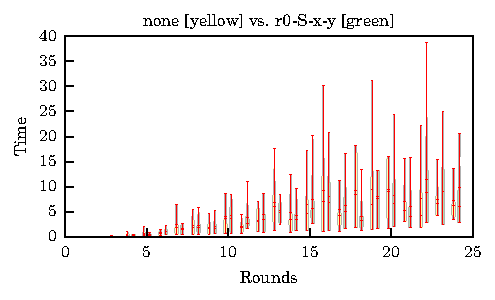
\includegraphics{figures/bo-ex1/sbs-time-none-r0sxy.pdf}
\caption{Violin plot comparing the solving time using two branching order strategies for $8$-bit SHA-3 preimage. For every number of rounds the left (yellow) violin shows the distribution of running times with the \emph{none} strategy along with the median, mean and extreme values. The right (green) violin shows the same for the \emph{r0-S-x-y} strategy.}
\label{fig:bo-sbs-time-none-r0sxy}
\end{figure}

\begin{figure}
\centering 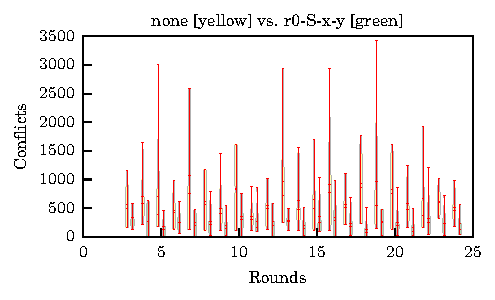
\includegraphics{figures/bo-ex1/sbs-confl-none-r0sxy.pdf}
\caption{Violin plot comparing the number of conflicts for two branching order strategies.}
\label{fig:bo-sbs-confl-none-r0sxy}
\end{figure}


For \emph{SHA-3-512} we tested various branching orders on $8$-bit reference preimage attack with number of rounds ranging from $0$ to $24$ (full SHA-3).
For every number of rounds 10 different instances were generated and each was solved 10 times, for a total of 100 samples per round per strategy.
We compared the following branching order strategies:

\textbf{\emph{none}}: No branching order was specified. This is the default unmodified \emph{MiniSat} behavior.

\textbf{\emph{r0-S-x-y}}: The $S$ matrix from the first round is branched on first, in column-major order.

\textbf{\emph{r0-S-y-x}}: Same as previous one, but in row-major order.

\textbf{\emph{rlast-S-x-y}} and \textbf{\emph{rlast-S-y-x-}}: Same as previous two, but the $S$ matrix from the last round is used instead.	

A plot comparing the solving time of the first two strategies is show in figure \ref{fig:bo-sbs-time-none-r0sxy}.
Figure \ref{fig:bo-sbs-confl-none-r0sxy} compares the number of conflicts.

We can see that the number of conflicts was reduced using the \emph{r0-S-x-y} strategy.
However the effect on solving time is harder to interpret -- while we can see the extremes for some rounds got better and for others they got worse, the distributions are too similar to see the effect.

\begin{figure}
\centering 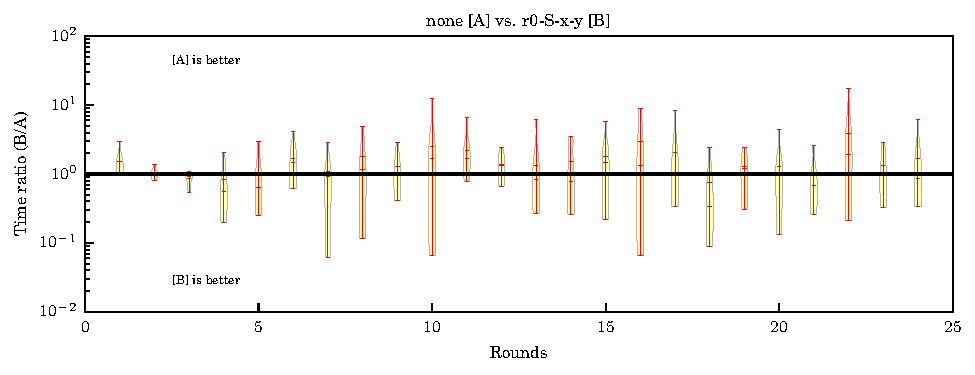
\includegraphics{figures/bo-ex1/ratio-time-none-r0sxy.pdf}
\caption{Violin plot showing the distribution of time ratios.}
\label{fig:bo-ratio-time-none-r0sxy}
\end{figure}

\begin{figure}
\centering 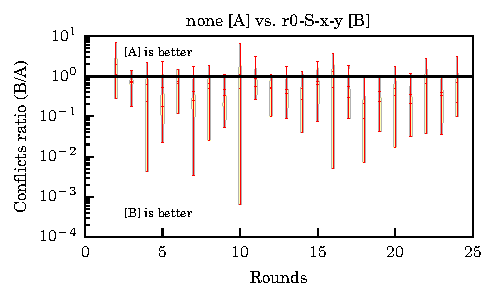
\includegraphics{figures/bo-ex1/ratio-confl-none-r0sxy.pdf}
\caption{Violin plot showing the distribution of number of conflict ratios.}
\label{fig:bo-ratio-confl-none-r0sxy}
\end{figure}


Instead we can plot the ratios of solving time and number of conflicts as in figures \ref{fig:bo-ratio-time-none-r0sxy} and \ref{fig:bo-ratio-confl-none-r0sxy}.
Here the violins show distributions of values that were obtained by taking pairs of samples (the solving time on some instance with one strategy and the solving time on that same instance with a different strategy) and taking their ratios.

From these plots we see that while the ratios for the number of conflict are mostly below 1 (meaning that the \emph{r0-S-x-y} strategy leads to fewer conflicts), the time ratios are often higher than 1.

TODO Games-Howell tabulky

The \emph{r0-S-y-x} strategy behaves the same as \emph{r0-S-x-y} -- the number of conflicts for every instance is identical and the differences in time are negligible.

TODO preco?

On the other hand the strategies starting with the last round's $S$ matrix lead to the same behavior as not providing any branch ordering at all (the \emph{none} strategy).
This must mean that either their choice does not lead to any forced assignments and conflicts (which is highly unlikely) or that the default \emph{MiniSat} heuristic is also picking them for branching first.

TODO debug printf do minisatu, zistit ktore z tohto sa deje

	
%A possible branch ordering would be based on the rounds of a hash function.
%Given the reduced 20 rounds variant of SHA-1, we could first force the solver to assign values to all variables corresponding to variables in the $n$-th round of the compression function.
%
%By trying various orders we obtain the results shown in Figure \ref{fig:opt-branchorder-example-sha1}-branchorder-example-sha1}.
%The numbers in the \emph{order} column refer to the rounds of the compression function.
%For example \emph{20, 19} means that first all variables from the 20th round get assigned, then all variables from 19th round and then the original heuristic takes over.
%
%While the times are averages over multiple runs they are still quite small and susceptible to random noise.
%However the number of conflicts is a more reliable measure and we can see interesting trends from this small example.
%Forcing the SAT solver to work backwards (20, 19, 18) is much worse than the general heuristic.
%On the other hand, starting with the first round leads to significant speed-up.
%
%\begin{figure}
%\caption{Solving time and number of conflicts for 8-bit preimage with 32-bit message on reduced 20-rounds SHA-1 with various branching orders.}
%\label{fig:opt-branchorder-example-sha1}
%\begin{tabular}{l|c|c}
%Order & Time [s] & Conflicts \\ \hline
%--- & 0.96 & 9755 \\ \hline
%20 & 0.94 & 9755 \\
%20, 19 & 0.97 & 9755 \\
%20, 19, 18 & 17.35 & 71197 \\ \hline
%1 & 0.35 & 1062 \\
%2 & 0.35 & 1062 \\
%1, 2 & 0.33 & 1062 \\
%1, 2, 3 & 0.29 & 927 \\
%1, 2, 3, 4 & 0.28 & 185 \\
%1, 4 & 0.24 & 119
%\end{tabular}
%\end{figure}
%TODO nicer table, new numbers with averages
%TODO rerun these numbers with more rounds? with more trials for better averages? and (!!!) with equal seed distributions (generate ~1k seeds, run each order with the same ones)
%TODO proper systematic evaluation
%TODO implement groups for branch ordering? might be slower due to complex selection...